%! TEX root = **/000-main.tex
% vim: spell spelllang=en:

\subsection{Non-Normalized arcsine kernel}

Now, we will introduce the non-normalized arcsine kernel, and compare it with
both the normalized arcsine kernel and the radial basis kernel.

\subsubsection{Regression}

\Cref{fig:nrmse-all-scaled} shows the nRMSE for all datasets using the normalized
and non-normalized arcsine kernels. We can observe that for values of $\sigma$
greater than $10^5$, the normalized and non-normalized arcsine kernels perform
similarly.

\begin{figure}[H]
    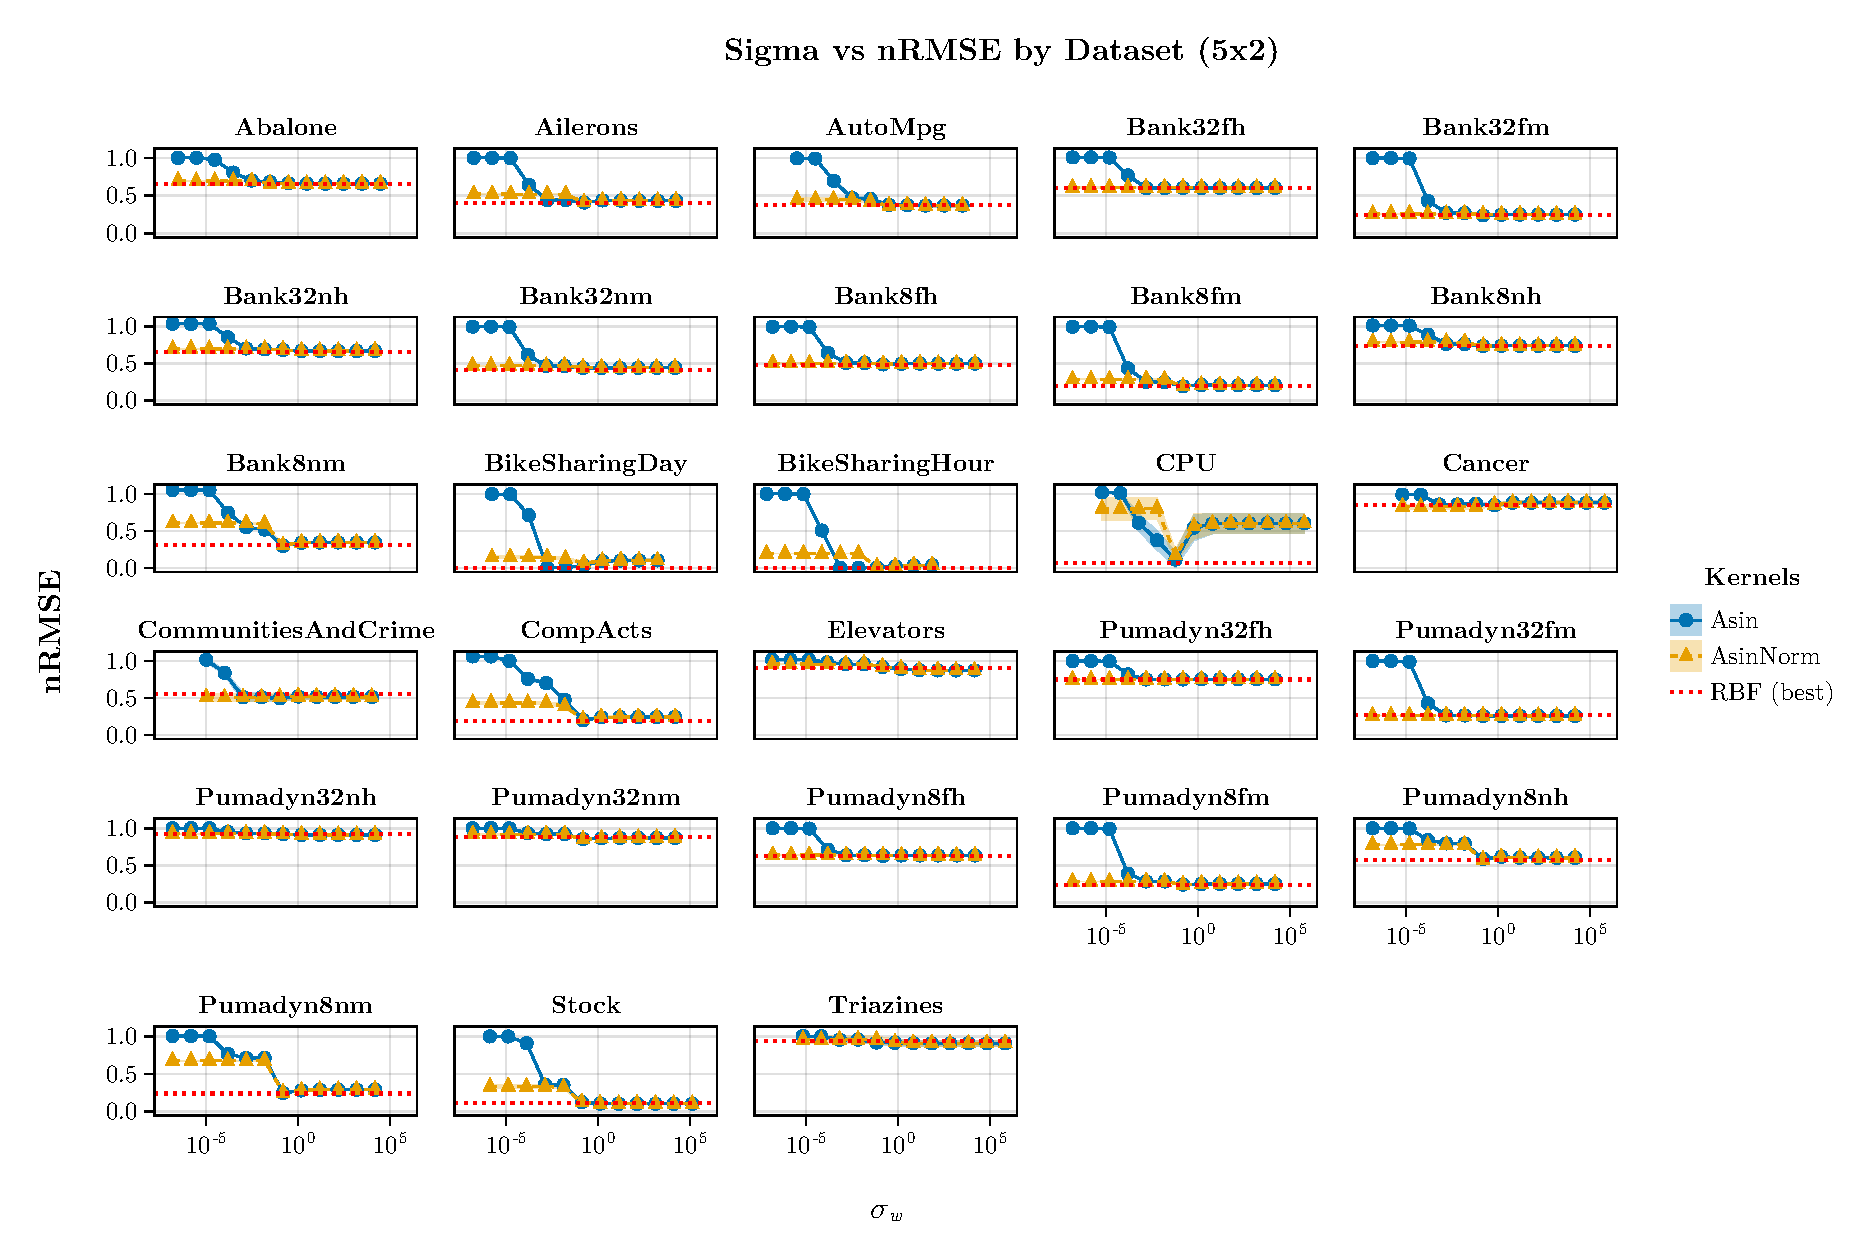
\includegraphics[width=\textwidth]{plots/nRMSE_all_scaled}
    \caption{Sigma vs Normalized Root Mean Squared error by dataset using Normalized and Non-Normalized arcsine kernel}%
    \label{fig:nrmse-all-scaled}
\end{figure}

% \begin{figure}[H]
%     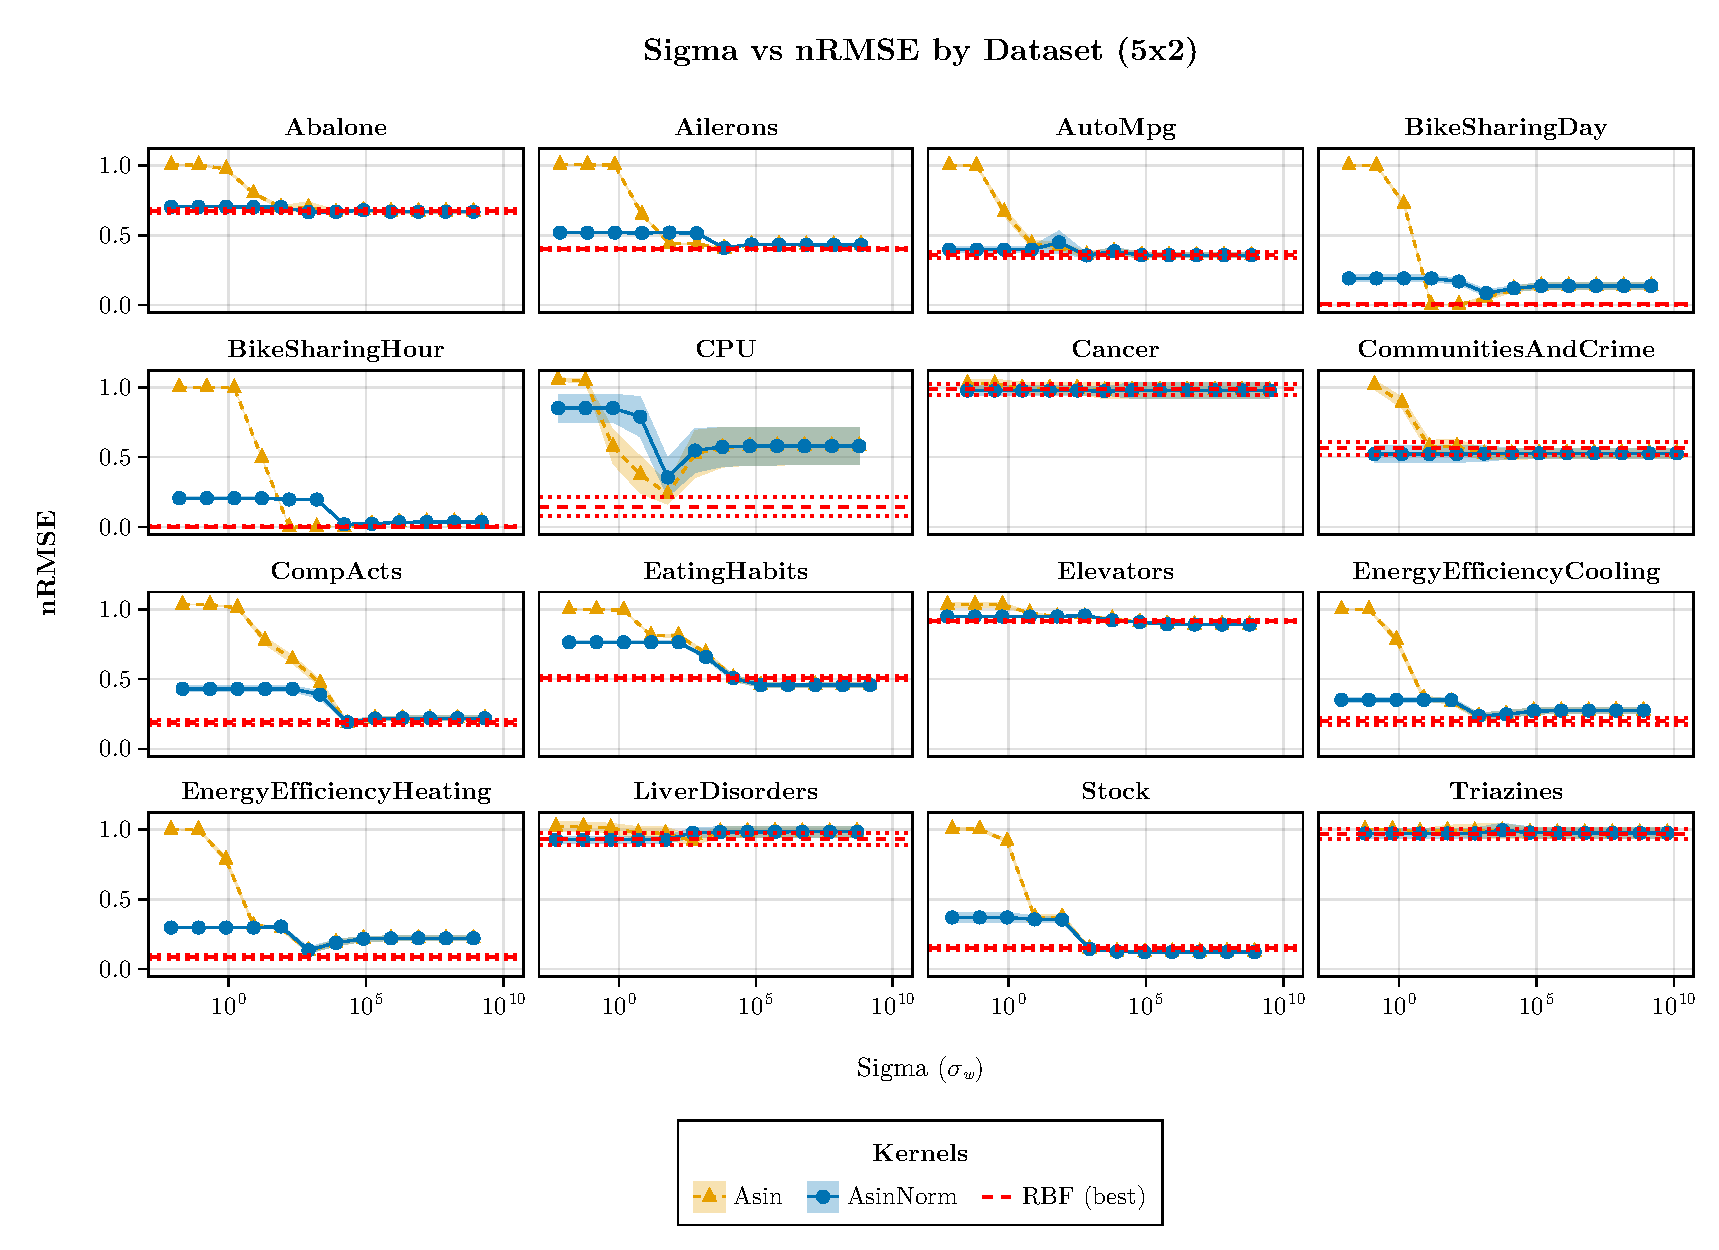
\includegraphics{plots/nRMSE_nodelve_all_scaled}
%     \caption{Sigma vs Normalized Root Mean Squared error by dataset using Normalized arcsine kernel}%
%     \label{fig:nrmse-all-scaled}
% \end{figure}

\subsubsection{Paired t-test}

\Cref{fig:paired-ttest-asin-asinnorm} shows the $p$\textendash{}values of the paired t-test
between the normalized and non-normalized arcsine kernels%
\footnote{A plot with the difference in \emph{nRMSE} similar to
    what we showed for rbf can be found in \cref{fig:paired-ttest-asin-asinnorm-diff} in the appendix.}%
, it follows the same
format described in \cref{ssub:comparison_with_radial_basis_rbf_kernel}.

\begin{figure}[H]
    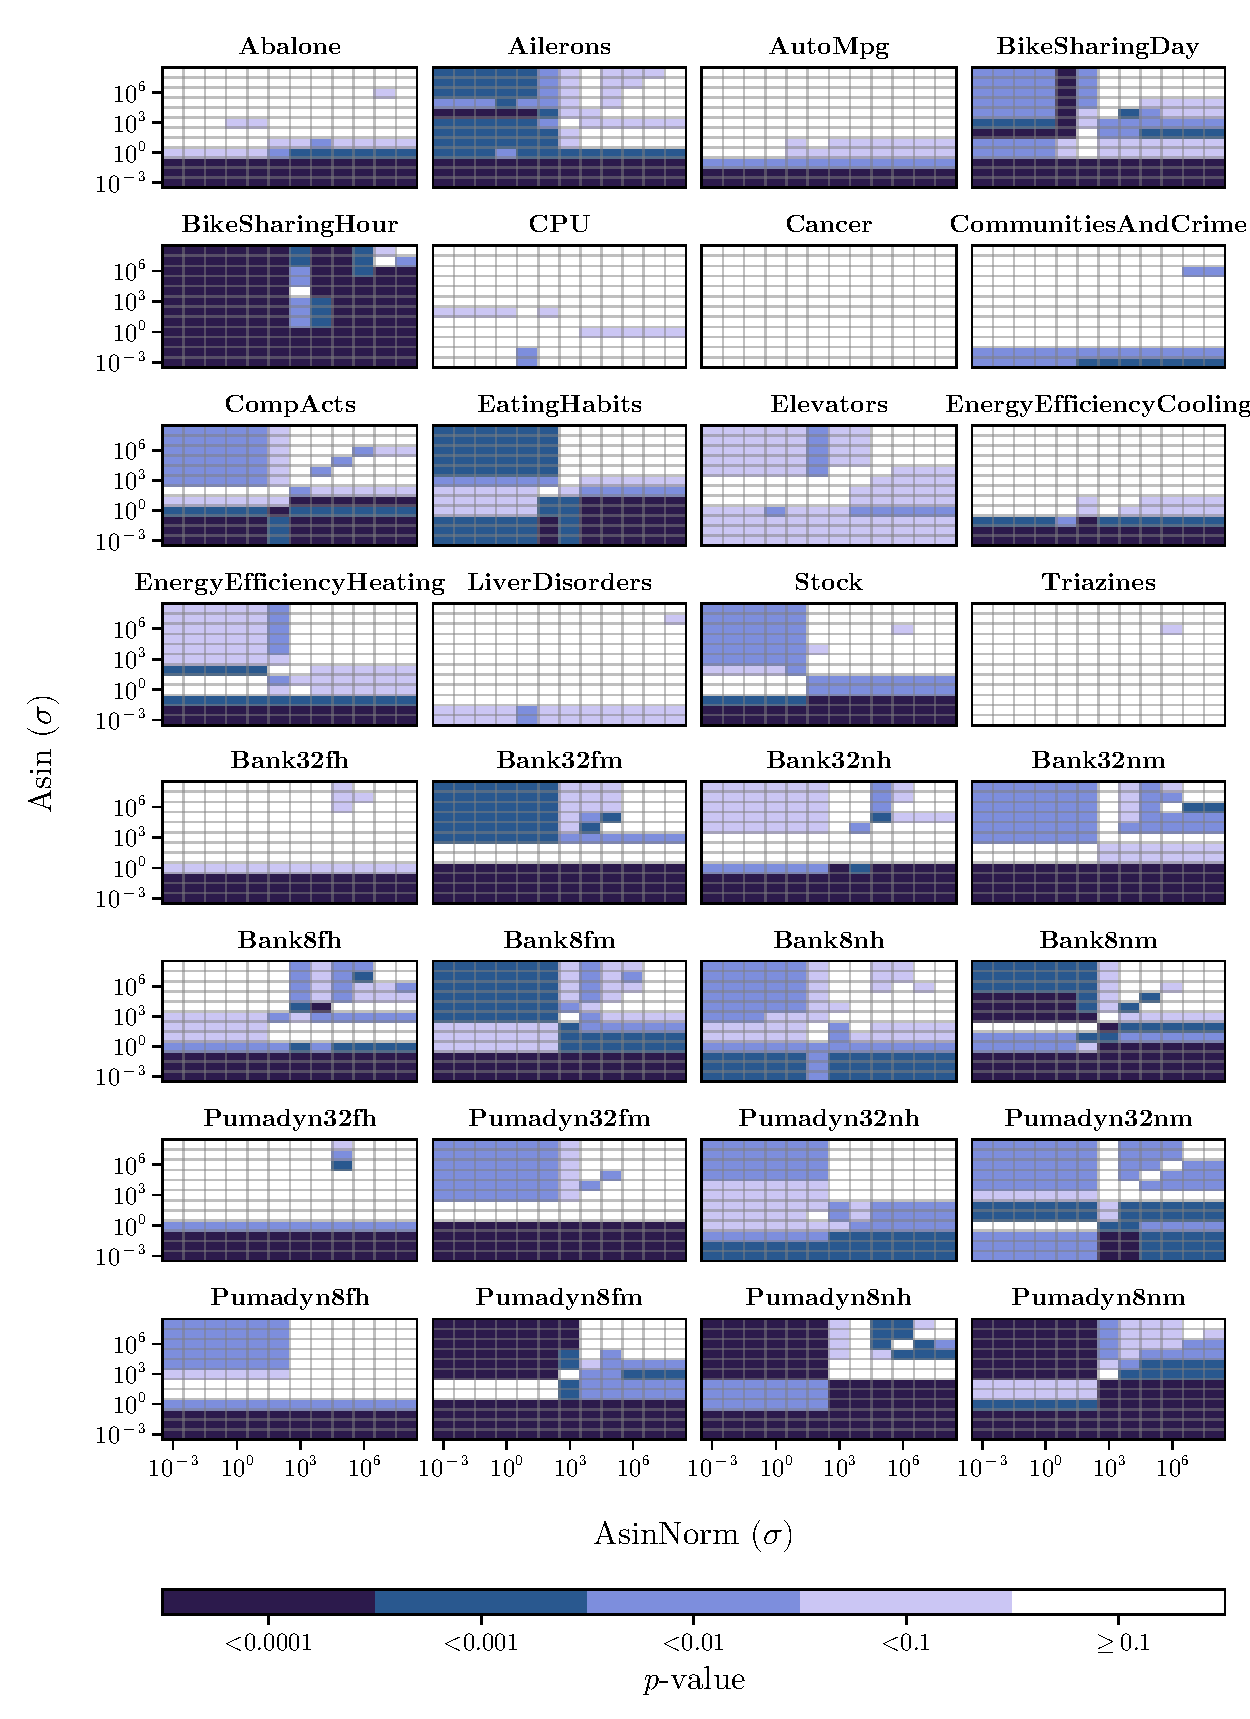
\includegraphics[width=0.9\textwidth]{plots/heatmaps_asin_asinnorm_pvalues}
    \caption{Paired t-test $p$\textendash{}values between normalized and non-normalized arcsine kernels}%
    \label{fig:paired-ttest-asin-asinnorm}
\end{figure}

The top right corner of all the plots in \cref{fig:paired-ttest-asin-asinnorm} shows
that for $\sigma = 10^6$, the $p$\textendash{}values are greater than $0.1$ for all datasets,
which means that the null hypothesis cannot be rejected, and therefore we cannot reject
the hypothesis that they both perform the same. This would indicate that our suspicion
that the normalization of the arcsine kernel is not necessary for large values of
$\sigma$ holds.

\subsubsection{Computational Cost}

If we naively compare the computational cost of the normalized and non-normalized
arcsine kernels by averaging the time or the number of iterations for all datasets,
some unexpected results appear. If we do the mean execution time for each kernel,
we find that the normalized arcsine kernel is 2 times slower than the non-normalized,
and it takes 4 times more iterations to converge.

However, upon closer inspection, upon closer inspection, we can see that the data
for the non-normalized arcsine kernel is skewed by the effects of the results for
small values of $\sigma$ ($\sigma < 10$). As we can see in \cref{fig:nrmse-all-scaled},
for such values the results obtained by the non-normalized arcsine kernel are
significantly worse than the normalized arcsine kernel (even \emph{nRMSE} = 1).
In these situations, the non-normalized arcsine kernel ends much faster than the
normalized arcsine kernel, but the results are extremely underwhelming.

If we only consider the results for $\sigma > 100$, we obtain a speedup
of 1.43 with the non-normalized arcsine kernel with respect to the normalized
version. In relation to the RBF kernel the speedup is 0.97, which means that
the non-normalized arcsine kernels is slightly slower than the RBF kernel in
average. Another interesting fact is that the number of iterations for the
arcsine kernel and the normalized arcsine kernel is almost the same for these
cases ($\sigma > 100$). Which further reinforces our hypothesis that the
normalization of the arcsine kernel is not necessary for large values of sigma.
